% Author-review manuscript. Evidence boundary and source map: README.md and WRITING_NOTES.md.
% The reference draft supplies the writing/typographic model, not performance values.
\documentclass[runningheads]{llncs}
\usepackage[T1]{fontenc}
\usepackage{amsmath}
\usepackage{newtxtext}
\usepackage[varvw]{newtxmath}
\usepackage{booktabs,array}
\usepackage{graphicx}
\usepackage{tikz}
\usetikzlibrary{arrows.meta,positioning,fit,calc}
\usepackage[hidelinks]{hyperref}
\providecommand{\Description}[1]{}
\newcommand{\method}{TitanTPP}
\newcommand{\GELU}{\operatorname{GELU}}
\newcommand{\softplus}{\operatorname{softplus}}
\newcommand{\Nrm}{\operatorname{norm}}
\newcommand{\Hcal}{\mathcal{H}}
\newcommand{\pmval}[2]{\ensuremath{#1\,{\scriptstyle\pm}\,#2}}
\definecolor{enc}{RGB}{226,237,248}
\definecolor{hist}{RGB}{218,239,231}
\definecolor{head}{RGB}{249,237,212}
\definecolor{ink}{RGB}{44,63,78}

\begin{document}
\title{TitanTPP: Local and Recurrent History Correction\texorpdfstring{\\}{ }for Event Quantity Prediction}
\titlerunning{TitanTPP: History Correction for Event Quantity Prediction}
\author{Anonymous Authors}
\authorrunning{Anonymous Authors}
\institute{Affiliations withheld for anonymous review}
\maketitle

\begin{abstract}
Event forecasting requires predicting how much will occur as well as when it will occur. A history encoder supplies information for both predictions, but this does not establish whether a separate path through recent observed states is useful. We study this question in TitanTPP, a causal attention model with an explicit correction path. The representative architecture applies a three-position correction to queries, keys, and values, then adds a gated recurrent residual between attention blocks. A separate comparison examines prototype retrieval with time and quantity queries. In a completed 54-run study of an earlier MLP correction, adding the correction reduced validation quantity RMSE in all 18 paired comparisons across three datasets. The benefit was largest on Taxi, where mean RMSE fell by 13.0--14.1\%, but recorded-time likelihood deteriorated. Prototype addition was less consistent. These findings motivate controls that separate previous-state input from additional parameters, and split-query retrieval from general query learning. The CNN+GRU controls remain under evaluation. We report the completed MLP comparison and one supplementary Instacart fit as development-validation evidence.
\keywords{Event forecasting \and Quantity prediction \and History correction \and Temporal point processes}
\end{abstract}

\section{Introduction}
A demand forecast must often answer two questions: when will the next event occur, and how large will it be? The answers are related, but errors in them have different consequences. A model may estimate ordinary events well while missing the quantities that dominate replenishment or capacity decisions. It may also improve quantity estimates at the expense of timing likelihood. Joint prediction therefore calls for an account of both outcomes, even when quantity is the primary objective.

Neural event models represent observed history through recurrence, attention, or a continuous-time state. RMTPP learns a recurrent history embedding~\cite{du2016rmtpp}; attentive neural Hawkes models use time-conditioned attention~\cite{yang2022anhp}; S2P2 uses a continuous-time state-space formulation~\cite{chang2025s2p2}. Such encoders already carry information about earlier events. The question here is narrower than whether history matters: \emph{does an explicit correction through recent observed states help after a history-aware encoder is already in place?}

We investigate this question with \method. The representative CNN+GRU54 model combines two forms of correction. A local path adjusts attention queries, keys, and values using the current and two preceding observed positions. A recurrent path adds a projected GRU state between the two attention blocks. The suffix 54 denotes the GRU state width. Both paths are residual, allowing the initial model to retain the shared encoder computation. They provide a particular way to reuse history, rather than supplying information unavailable to the causal encoder.

An earlier MLP version gives a reason to examine the correction more closely. Across Taxi, Intermittent, and RAF Spare Parts, switching on its explicit previous-state path improved overall quantity RMSE in all 18 comparisons formed by three seeds and two prototype settings. Yet the strongest quantity gains came with worse timing likelihood on Taxi. Moreover, adding prototypes to the corrected model did not improve quantity RMSE consistently across datasets. This pattern motivates two separate questions: the value of an explicit history path, and the value of the rule used to retrieve from a learned prototype bank.

The distinction matters for attribution. Removing the history path also removes parameters, so that comparison alone cannot identify the benefit of its input. We therefore include a control with the same number of active correction parameters that operates only on the current position. For retrieval, we compare uniform averaging, similarity weighting, separately normalized time and quantity queries, and a general learned query. Only the last two introduce query parameters, and their budgets are matched. The encoder, output heads, and model-selection rule are shared in each study.

This paper makes three contributions:
\begin{enumerate}
\item We describe a local and recurrent correction architecture for next-event quantity prediction within a causal attention model, including the observation rules that prevent access to the target event.
\item We formulate controlled comparisons for explicit history input and prototype retrieval, separating these questions from extra parameter count and from the choice of output distribution.
\item We report the completed MLP correction study, including seed consistency, large-quantity errors, and timing tradeoffs. Its results support further testing of explicit correction, while showing why quantity improvements alone do not establish a uniformly better event model.
\end{enumerate}
The empirical analysis in this version concerns the MLP study. The representative CNN+GRU comparisons and the supplementary Instacart architecture comparison are specified separately, so that a result for one architecture is not treated as evidence for another.

\section{Related Work}
\paragraph{Encoding event history.}
RMTPP embeds marked event history with a recurrent network and conditions the next event on that representation~\cite{du2016rmtpp}. Transformer attention provides a different route for combining sequence states~\cite{vaswani2017attention}, and attentive neural Hawkes models adapt attention to irregular event times~\cite{yang2022anhp}. More recently, S2P2 models marked event sequences through a continuous-time state-space model~\cite{chang2025s2p2}. These approaches differ in how history evolves and how it is read at prediction time. Our study holds a causal attention backbone fixed and asks whether an additional local and recurrent path is useful within it. A recurrent correction is not, by itself, a new class of history encoder.

\paragraph{Event size and timing.}
Deep renewal processes jointly address intermittent event occurrence and demand size~\cite{turkmen2021renewal}. This is particularly relevant when the mark is a quantity rather than a category. Our evaluation emphasizes raw quantity error and reports timing likelihood at the same selected checkpoint. The recorded intervals are discrete, so the time head assigns probability mass to recorded bins rather than evaluating a continuous density at an integer. Comparisons with other event models must retain this distinction: a common-head adaptation and a model's native marked-event likelihood answer different evaluation questions.

\paragraph{Learned memory and retrieval.}
Persistent memory augments self-attention with learned, input-independent key--value entries~\cite{sukhbaatar2019memory}. Product-key memory likewise retrieves learned values from a parameterized memory~\cite{lample2019product}. \method{} uses persistent entries inside attention and a separate bank of 64 learned prototypes after the encoder. The latter is a static parameter bank, not a store of past event records. Our retrieval question concerns the query: whether separately normalizing time and quantity views helps compared with a joint learned query using the same summaries. Top-$k$ selection and learned memory slots are established components of this design.

\section{Method}
\subsection{Prediction Task and Causal Encoder}
Let $\Hcal_j=\{(\Delta_i,q_i)\}_{i\leq j}$ be an observed event prefix, where $\Delta_i$ is an inter-event interval and $q_i\geq0$ is an event quantity. The model predicts the recorded interval $D_{j+1}$ and quantity $q_{j+1}$ of the next event. The target position is withheld from the input, and the prediction is read from the last observed position $j$. Padding is not an event.

Each observed event is embedded as
\begin{equation}
 e_i=W_e[\log(1+\Delta_i),\log(1+q_i)]^\top+b_e+p_i,
\end{equation}
where $p_i$ is a learned position embedding. These two input values are not standardized by training-set moments. The backbone has two pre-normalized causal attention blocks, hidden width 64, four attention heads, a feed-forward width of 128, and dropout 0.1. Each block also contains 16 learned persistent key--value entries. These entries are distinct from the prototype bank used after the encoder.

Figure~\ref{fig:architecture} shows where the corrections enter. In the first block, the local correction is applied after layer normalization and the query, key, and value projections, before causal attention. The block then completes its attention residual and feed-forward residual. Its output $b_i$ is passed through the recurrent correction before entering the second block. Let $h_i$ denote the resulting second-block output.

\begin{figure}[t]
\centering
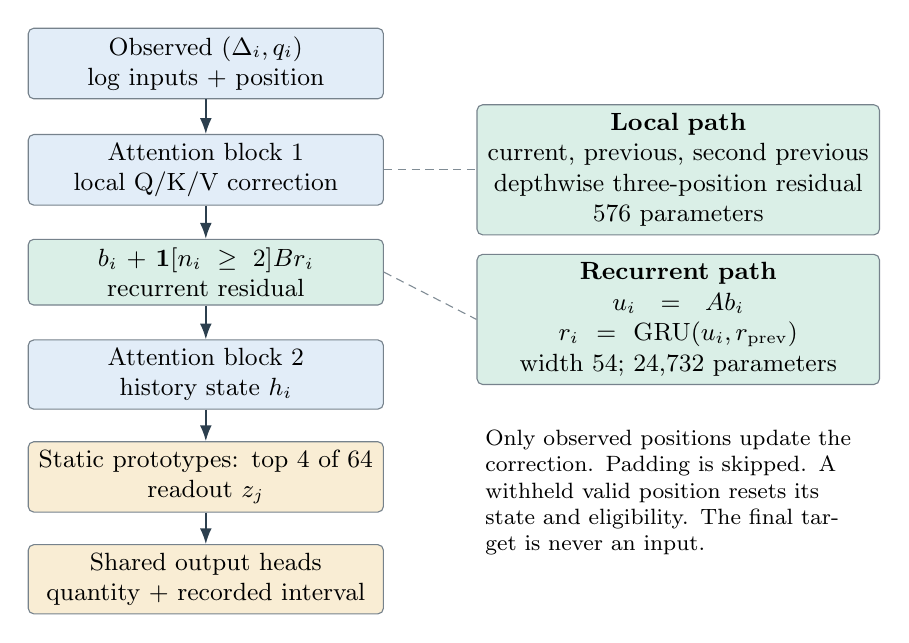
\begin{tikzpicture}[font=\small,>=Latex,
 box/.style={draw=ink!65,rounded corners=2pt,align=center,minimum height=8mm,text width=43mm,inner sep=3pt},
 flow/.style={->,draw=ink,semithick}]
\node[box,fill=enc] (input) at (0,0) {Observed $(\Delta_i,q_i)$\\log inputs + position};
\node[box,fill=enc] (first) at (0,-1.35) {Attention block 1\\local Q/K/V correction};
\node[box,fill=hist] (res) at (0,-2.65) {$b_i+\mathbf{1}[n_i\geq2]Br_i$\\recurrent residual};
\node[box,fill=enc] (second) at (0,-3.95) {Attention block 2\\history state $h_i$};
\node[box,fill=head] (proto) at (0,-5.25) {Static prototypes: top 4 of 64\\readout $z_j$};
\node[box,fill=head] (heads) at (0,-6.55) {Shared output heads\\quantity + recorded interval};
\foreach \a/\b in {input/first,first/res,res/second,second/proto,proto/heads}
 \draw[flow] (\a) -- (\b);
\node[box,text width=49mm,fill=hist] (local) at (6,-1.35) {\textbf{Local path}\\current, previous, second previous\\depthwise three-position residual\\576 parameters};
\node[box,text width=49mm,fill=hist] (gru) at (6,-3.25) {\textbf{Recurrent path}\\$u_i=A b_i$\\$r_i=\mathrm{GRU}(u_i,r_{\rm prev})$\\width 54; 24,732 parameters};
\node[align=left,text width=49mm,font=\footnotesize] at (6,-5.45) {Only observed positions update the correction. Padding is skipped. A withheld valid position resets its state and eligibility. The final target is never an input.};
\draw[densely dashed,draw=ink!60] (first.east) -- (local.west);
\draw[densely dashed,draw=ink!60] (res.east) -- (gru.west);
\end{tikzpicture}
\caption{CNN+GRU54 in \method. The local correction operates within the first attention block; the recurrent correction operates between blocks. Prototype retrieval and the two output heads follow the encoder. The correction paths contain 25,308 parameters in total.}
\label{fig:architecture}
\Description{A vertical causal encoder pipeline with enlarged local and recurrent correction modules to its right.}
\end{figure}

\subsection{Local and Recurrent History Correction}
For a projected query, key, or value sequence $X$, the local path computes
\begin{equation}
 \widetilde X_i=X_i+\sum_{\ell=0}^{2}a_{i\ell}\,\kappa^X_\ell\odot X_{s_\ell(i)}.
 \label{eq:local}
\end{equation}
Here $s_0(i)=i$, and $s_1(i),s_2(i)$ are the preceding observed positions in the same correction segment. The mask $a_{i\ell}$ indicates that the corresponding position exists. Each $\kappa^X_\ell\in\mathbb{R}^{64}$ acts channelwise. Applying this three-position operation to queries, keys, and values uses $3\times3\times64=576$ parameters. The operation permits nearby observed states to alter the attention inputs without replacing the attention layer itself.

The recurrent path projects the first-block output into a 54-dimensional state:
\begin{equation}
 u_i=A b_i,\qquad r_i=\mathrm{GRU}(u_i,r_{\mathrm{prev}}),\qquad
 \widetilde b_i=b_i+\mathbf{1}[n_i\geq2]B r_i.
 \label{eq:recurrent}
\end{equation}
The GRU follows the gated recurrent formulation~\cite{cho2014gru}; $A$ and $B$ are bias-free projections, and $n_i$ counts observed events in the current correction segment. The residual uses the state \emph{after} processing event $i$. The recurrent path has 24,732 parameters, including its projections. Its state width is independent of the number of observed events.

Padding neither updates the GRU nor advances the observation count. A valid but withheld position resets the correction state and its eligibility masks. This reset concerns the correction path; it does not change the causal attention mask into a segment-reset mask. The local kernels and recurrent output projection $B$ are initialized to zero. Thus the correction initially leaves the shared encoder computation unchanged, while its input and recurrent parameters can still be learned.

\paragraph{What the controls isolate.}
The correction-removal variant bypasses both optional paths. The current-only control retains their parameter shapes, initialization, and observation-count masks, but removes direct reads of earlier positions. In Eq.~\eqref{eq:local}, the three bases become $X_i$, $\tanh(X_i)$, and $\GELU(X_i)$, with the original one-, two-, and three-observation eligibility. For the recurrent component, the current-only control starts from zero at each position and applies two GRU updates using the same current input $u_i$. Its projected output is used only when $n_i\geq2$.

The full and current-only paths both contain 25,308 active correction parameters. Their computations nevertheless differ: the current-only control uses nonlinear bases and repeated current-input updates. It also receives $b_i$, which already summarizes a prefix through attention. Consequently, this comparison isolates a particular explicit history path against a current-position path; it does not compare a model with history against one without history, or identify the effect of a single lag in isolation.

\subsection{Static Prototype Retrieval}
After the encoder, a learned bank $M=\{m_k\}_{k=1}^{64}$ supplies a residual to the last observed state $h_j$. Each slot $m_k\in\mathbb{R}^{64}$ serves as both key and value: its normalized vector is used for scoring, and its raw vector is added to the readout. The slots are fitted with the rest of the model and are not written with observed events at inference time.

Let $\Nrm(x)=x/\max(\|x\|_2,\epsilon)$ and let $S_j$ contain the four highest-scoring slots. The mean baseline uses cosine scores $s_{jk}=\Nrm(h_j)^\top\Nrm(m_k)$ and uniform weights. The weighted variant retains these scores but applies a softmax within the selected four:
\begin{equation}
 z_j=h_j+\sum_{k\in S_j}\alpha_{jk}m_k,\qquad
 \alpha_{jk}=\frac{\exp(s_{jk})}{\sum_{v\in S_j}\exp(s_{jv})}.
 \label{eq:readout}
\end{equation}
Mean retrieval instead sets $\alpha_{jk}=1/4$. Neither variant introduces additional query parameters.

The two learned-query variants receive summaries of the most recent 32 observed positions in the current correction segment, including the current event. Time summaries use standardized $\log(\Delta/s)$; quantity summaries use standardized $\log(1+q)$, with moments computed from training observations. Each four-dimensional view contains the latest value, mean, population standard deviation, and difference between the latest two eligible values. Nonpositive gaps are excluded from time summaries, whereas zero quantities are retained. The standard deviation and difference require two eligible observations; unavailable summaries are zero. Denote the resulting views by $\phi_t$ and $\phi_q$.

The fixed split-query rule forms
\begin{align}
 v_t&=h_j+\phi_t W_t, & v_q&=h_j+\phi_q W_q,\\
 s^{\mathrm{fixed}}_{jk}
 &=\tfrac12\Nrm(v_t)^\top\Nrm(m_k)
   +\tfrac12\Nrm(v_q)^\top\Nrm(m_k).
 \label{eq:fixed}
\end{align}
The two $4\times64$ projections contain 512 parameters. A budget-matched general-query control uses the same eight summaries, with
\begin{equation}
 v_g=h_j+\tfrac12[\phi_t,\phi_q]W_g,\qquad
 s^{\mathrm{general}}_{jk}=\Nrm(v_g)^\top\Nrm(m_k),
 \label{eq:generic}
\end{equation}
where $W_g\in\mathbb{R}^{8\times64}$. Both variants use Eq.~\eqref{eq:readout}, temperature one, and zero-initialized query projections. Figure~\ref{fig:retrieval} highlights the difference: separate normalization before score averaging versus normalization after the two views have been combined.

\begin{figure}[t]
\centering
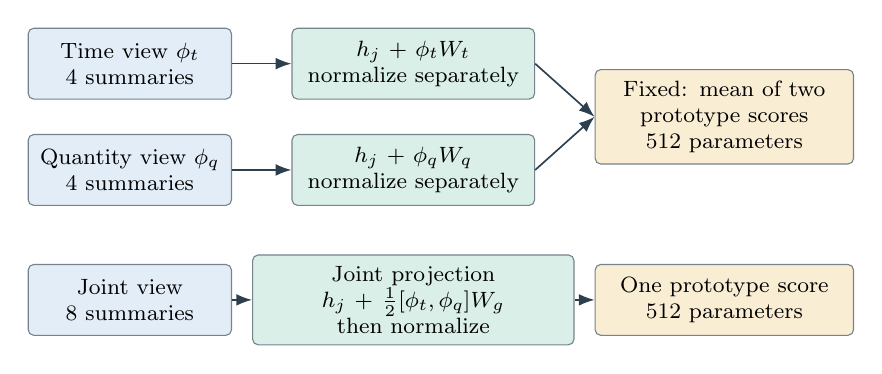
\begin{tikzpicture}[font=\footnotesize,>=Latex,
 b/.style={draw=ink!65,rounded corners=2pt,align=center,inner sep=4pt,minimum height=9mm},
 a/.style={->,semithick,draw=ink}]
\node[b,fill=enc,text width=23mm] (t) at (0,0) {Time view $\phi_t$\\4 summaries};
\node[b,fill=enc,text width=23mm] (q) at (0,-1.35) {Quantity view $\phi_q$\\4 summaries};
\node[b,fill=hist,text width=28mm] (tn) at (3.6,0) {$h_j+\phi_tW_t$\\normalize separately};
\node[b,fill=hist,text width=28mm] (qn) at (3.6,-1.35) {$h_j+\phi_qW_q$\\normalize separately};
\node[b,fill=head,text width=30mm] (f) at (7.55,-.675) {Fixed: mean of two\\prototype scores\\512 parameters};
\draw[a] (t) -- (tn); \draw[a] (q) -- (qn);
\draw[a] (tn.east) -- (f.west); \draw[a] (qn.east) -- (f.west);
\node[b,fill=enc,text width=23mm] (joint) at (0,-3) {Joint view\\8 summaries};
\node[b,fill=hist,text width=38mm] (g) at (3.6,-3) {Joint projection\\$h_j+\tfrac12[\phi_t,\phi_q]W_g$\\then normalize};
\node[b,fill=head,text width=30mm] (gs) at (7.55,-3) {One prototype score\\512 parameters};
\draw[a] (joint) -- (g); \draw[a] (g) -- (gs);

\end{tikzpicture}
\caption{The matched retrieval comparison. Both rules select four of 64 prototypes and use softmax weights. The fixed rule constrains two normalized views to equal score contributions; the general query learns a joint projection before normalization.}
\label{fig:retrieval}
\Description{Separate normalized time and quantity queries compared with a joint normalized query, each with 512 additional parameters.}
\end{figure}

The fixed score also has a concatenated dot-product expression:
\begin{equation}
 \tfrac12[\Nrm(v_t),\Nrm(v_q)]^\top[\Nrm(m_k),\Nrm(m_k)].
\end{equation}
The comparison tests separate query normalization and fixed score mixing. The comparisons share an architecture, not fitted encoder or prototype values: every arm is trained end to end.

\subsection{Shared Output Heads and Training Objective}
The quantity head predicts in log space and is evaluated in raw units:
\begin{equation}
 \widehat\ell_j=\softplus(w_q^\top z_j+b_q),\qquad
 \widehat q_{j+1}=\exp(\widehat\ell_j)-1.
\end{equation}
No inverse training-set standardization is applied. The time head gives
\begin{equation}
 \mu_j=w_\mu^\top z_j+b_\mu,\qquad
 \sigma_j=10^{-3}+\softplus(w_\sigma^\top z_j+b_\sigma).
\end{equation}
For a dataset scale $s>0$, let $T=s\exp(\mu_j+\sigma_j\varepsilon)$ with $\varepsilon\sim\mathcal N(0,1)$ and $F_j(x)=\Phi((\log(x/s)-\mu_j)/\sigma_j)$. The recorded interval is $D=\max(1,\operatorname{round}T)$, so its probability mass is
\begin{equation}
 p_j(d)=
 \begin{cases}
 F_j(1.5),& d=1,\\
 F_j(d+0.5)-F_j(d-0.5),& d\geq2.
 \end{cases}
 \label{eq:time}
\end{equation}
For Instacart, the recorded interval is capped at 30 days: the interior-bin rule applies for $2\leq d<30$, and $p_j(30)=1-F_j(29.5)$. Training minimizes the sum of recorded-time negative log-likelihood and squared log-quantity error,
\begin{equation}
 \mathcal L=-\log p_j(D_{j+1})+
   \bigl(\widehat\ell_j-\log(1+q_{j+1})\bigr)^2.
\end{equation}
The quantity weight is one, with no extra large-quantity loss term. All compared arms use these heads and this objective.

\section{Experimental Design}
\subsection{Datasets and Model Selection}
Taxi, Intermittent, and RAF Spare Parts form the core study. Instacart provides a supplementary architecture comparison. Table~\ref{tab:data} gives the eligible target populations and input windows. Lookback is measured in each dataset's native time bins. The inclusive window ends at the last observed event; the target is appended before truncation to the sequence cap, which includes that target. Large-quantity thresholds are fixed from the training data.

\begin{table}[t]
\caption{Target populations and sequence construction. $q_{\rm large}$ is a strict lower bound for the large-quantity subset. Scale $s$ is used by the time distribution.}
\label{tab:data}
\centering\small
\setlength{\tabcolsep}{4pt}
\begin{tabular}{@{}lrrrllr@{}}
\toprule
Dataset & Training & Validation & Cap & Lookback & $q_{\rm large}$ & $s$\\
\midrule
Taxi & 38,393 & 8,268 & 256 & 168 hours & $3449$ & 1\\
Intermittent & 393,824 & 86,285 & 256 & 520 weeks & $187$ & 3\\
RAF & 25,779 & 6,690 & 84 & 84 months & $200$ & 6\\
Instacart & 1,991,192 & 503,733 & 64 & 52 days & $35$ & 7\\
\bottomrule
\end{tabular}
\end{table}

The representative experiments use AdamW~\cite{loshchilov2019adamw}, learning rate $10^{-3}$, weight decay 0.01, batch size 128, and gradient clipping at one. Training lasts at least 40 and at most 300 epochs, with patience 40. Each fit retains the first strictly improving finite minimum of overall raw-quantity RMSE on the full validation set. Ties retain the earlier checkpoint. This rule is shared by the completed MLP study and the new comparisons; neither timing likelihood nor large-quantity error changes the selected epoch.

We evaluate quantity RMSE, quantity MAE, and recorded-time NLL on all validation targets and on the large-quantity subset. All six metrics come from that one checkpoint. Three-seed summaries use the arithmetic mean and sample standard deviation. Time scores are interpreted within a dataset, since the recorded units and distributions differ.

\subsection{Comparisons and Their Scope}
\paragraph{Completed MLP correction study.}
The initial study crosses prototype removal/addition ($P_0/P_1$) with correction removal/addition ($H_0/H_1$), giving a $2\times2$ comparison. It places an MLP correction between the first and second attention blocks, with no local Q/K/V correction; prototype retrieval follows the second block. Thus it differs from both correction paths in CNN+GRU54. Eight bias-free branches each map the concatenated current and immediately preceding observed states through $128\!\to\!8\!\to\!64$, and their outputs are averaged. The branches become eligible after more than 1, 2, 4, 8, 16, 32, 64, or 128 observations. These are eligibility thresholds, not eight different history lags.

The correction contains 12,288 parameters; the 64-slot prototype bank contains 4,096. Two additional controls test alternatives to these components. $P_1H_C$ replaces the correction with eight current-state branches of width 12, matching its parameter count. $P_FH_1$ replaces the prototype residual with a bias-free $64\!\to\!32\!\to\!64$ feed-forward residual, also using 4,096 parameters. All six arms retain the backbone's persistent attention entries. The six arms, three datasets, and seeds 42, 52, and 62 produce 54 completed fits.

These budget controls have limits. The feed-forward substitute differs in activation and initialization from prototype retrieval. Equal parameter counts do not imply equal computation. On RAF, the sequence cap prevents the eighth MLP branch from becoming eligible, leaving seven potentially active branches. These details constrain what can be attributed to the nominal budgets.

\paragraph{Representative correction and retrieval studies.}
CNN+GRU54 is compared with correction removal and the current-only control on each core dataset and seed: 27 fits. The retrieval comparison adds weighted, fixed, and general-query variants, with the nine full-correction models reused as the mean baseline. This requires 27 further fits, rather than a second training of the same mean models. The matched general query has 512 added parameters; it is distinct from the 521-parameter control used in the earlier exploratory retrieval pilot.

For a dataset and seed, all comparison arms run on the same GPU and software environment. Taxi and RAF are assigned to RTX 5080; Intermittent to RTX 5090. A preliminary implementation check compared CNN+GRU54 with mean retrieval on RTX 5080: 83 bitwise checks covered initialization, synthetic sequences, and the first three updates on a shared Taxi training batch. This establishes a limited implementation baseline, not equivalence of past training trajectories or checkpoints obtained on another GPU.

On Instacart, the supplementary study compares MLP8, MLP12, and CNN+GRU54 across the same three seeds, adding nine fits. It asks about architecture behavior on a fourth dataset; it does not replace the correction or retrieval controls. Together, these studies specify 63 new fits. Their completed comparisons will determine the representative model's evidence, independently of the MLP findings below.

\paragraph{Decision criteria and computational cost.}
The correction criterion requires the full model to have lower overall quantity RMSE than both controls in every seed on the same two or more core datasets. The fixed-retrieval criterion requires corresponding improvements over mean, weighted, and the general-query control. These are descriptive consistency criteria, not significance tests.

Retrieval must also meet a predeclared cost bound relative to mean retrieval on the same GPU. With batch 128, sequence lengths 64 and 256, five warm-up iterations and twenty measured iterations, the allowed increases are 20\% for inference time, 30\% for training-step time, and 20\% for peak allocation. Both lengths must pass. Results from arms above these bounds remain part of the comparison.

\section{Results}
\subsection{Quantity Gains in the Completed MLP Study}
Table~\ref{tab:rmse} reports the complete six-arm quantity comparison. Adding the MLP correction reduces overall RMSE in all 18 paired comparisons: three datasets, three seeds, and two prototype settings. Without prototypes, the reductions in the means are 13.04\% on Taxi, 9.01\% on Intermittent, and 0.77\% on RAF. With prototypes, the corresponding reductions are 14.11\%, 3.28\%, and 0.85\%. The direction is consistent, but the magnitude is strongly dataset-dependent.

\begin{table}[t]
\caption{Completed MLP study: overall validation quantity RMSE (mean $\pm$ sample SD over three seeds; lower is better). Bold marks the lowest mean within each dataset. These are not CNN+GRU54 results.}
\label{tab:rmse}
\centering\small
\setlength{\tabcolsep}{6pt}
\begin{tabular}{@{}lccc@{}}
\toprule
Arm & Taxi & Intermittent & RAF\\
\midrule
$P_0H_0$ & \pmval{88.977}{0.501} & \pmval{1.777}{0.065} & \pmval{34.242}{0.147}\\
$P_1H_0$ & \pmval{90.509}{0.521} & \pmval{1.721}{0.045} & \pmval{34.230}{0.127}\\
$P_0H_1$ & $\mathbf{77.377}\,{\scriptstyle\pm}\,1.822$ & $\mathbf{1.617}\,{\scriptstyle\pm}\,0.009$ & \pmval{33.979}{0.045}\\
$P_1H_1$ & \pmval{77.735}{0.681} & \pmval{1.664}{0.009} & $\mathbf{33.938}\,{\scriptstyle\pm}\,0.071$\\
$P_FH_1$ & \pmval{79.255}{1.230} & \pmval{1.759}{0.124} & \pmval{34.125}{0.074}\\
$P_1H_C$ & \pmval{88.846}{1.267} & \pmval{1.728}{0.061} & \pmval{34.273}{0.327}\\
\bottomrule
\end{tabular}
\end{table}

The parameter controls provide a more selective result. $P_1H_1$ beats both $P_FH_1$ and $P_1H_C$ in all three seeds on Taxi and RAF. On Intermittent, it beats each control in only two of three seeds. Thus the original MLP study satisfies its two-dataset consistency criterion, while leaving an exception on Intermittent. The large Taxi gap against $P_1H_C$ is compatible with useful explicit previous-state input in this MLP architecture; the control does not establish which part of the CNN+GRU path would account for such an effect.

Prototype addition yields a different pattern. With the correction already present, $P_1H_1$ has 0.46\% higher mean RMSE than $P_0H_1$ on Taxi and 2.92\% higher RMSE on Intermittent. On RAF it improves the mean by 0.12\%. The completed evidence therefore favors explicit correction more consistently than prototype addition. Choosing a different best variant for each dataset would conceal this distinction and would not define a single representative model.

\subsection{Timing, Large Quantities, and Cost}
Quantity gains are not uniform gains across outputs. On Taxi, adding correction raises overall time NLL from 0.818 to 1.253 without prototypes and from 0.725 to 1.229 with prototypes. These are increases of 53.17\% and 69.64\% in the means; timing NLL worsens in every seed under both settings. The checkpoints were selected for quantity RMSE, so this is a tradeoff at the quantity-selected model rather than a comparison of separately optimized timing checkpoints.

Large-quantity behavior also qualifies the overall result. The Taxi full model has large-quantity RMSE 376.660, compared with 366.709 for its feed-forward prototype substitute, despite lower overall RMSE. On RAF, adding correction slightly reduces overall RMSE but increases large-quantity MAE by 1.27\% without prototypes and 0.94\% with prototypes. Its large-quantity time NLL rises by 3.64\% and 3.85\%, respectively. The large subsets contain only 79 Taxi targets and 50 RAF targets, compared with 1,141 on Intermittent. Appendix~\ref{app:metrics} retains all six metrics, including these unfavorable outcomes.

The historical technical checks do not show that prototype retrieval is cheaper than its parameter-matched substitute. On RTX 5080, the measured step time for $P_1H_1$ is 36.46\,ms versus 25.34\,ms for $P_FH_1$ at length 256, and 14.15\,ms versus 11.49\,ms at length 84. On RTX 5090 at length 256, the corresponding times are 23.11 and 17.74\,ms. These checks use the median of three synthetic optimizer steps, without discarded warm-up, and include gradient-copy and verification work. They are limited technical measurements, not pure throughput or inference benchmarks, and do not implement the new retrieval cost protocol.

\subsection{Evidence Available for the Representative Architecture}
The CNN+GRU correction and matched retrieval comparisons do not yet have completed results in the evidence used here. Their implementation and experimental controls are specified in Sections 3 and 4, but the MLP results cannot establish their effects.

The archived observation of 8 October 2026, 14:38 KST contains one completed Instacart fit: MLP8, seed 52, on RTX 5090. It selected epoch 15 and stopped after epoch 55, with overall quantity RMSE 5.884, MAE 3.994, and time NLL 2.812. For the 6,036 large-quantity targets, the same checkpoint gives RMSE 24.665, MAE 22.088, and time NLL 2.900. This is a single-fit observation, not a three-seed architecture comparison; final collection of the complete stage remains outstanding. It cannot rank MLP8, MLP12, and CNN+GRU54.

\section{Discussion}
The completed study gives a specific empirical motivation for explicit correction. Quantity RMSE improves consistently when the MLP path is added, and the full model beats the two budget controls in every seed on two datasets. At the same time, prototype addition is not consistently helpful, and the largest correction gains coincide with a timing penalty. These results argue for separating the two mechanisms and for keeping timing and large-quantity errors visible alongside the primary metric.

The representative architecture changes the correction mechanism substantially. Its local operation reads three observed positions, while its GRU carries a recurrent state across the observed prefix. A successful full-versus-current-only comparison would support that combined path, not a claim that one preceding state alone explains the gain. Equal active parameter counts narrow the capacity explanation but do not remove differences in operations, depth, or optimization. Component-level attribution would require further controls.

The retrieval hypothesis is narrower still. Fixed split-query scoring can be expressed as a concatenated dot product. A benefit over the matched general query would support the tested separate-normalization constraint, not the invention of a fundamentally new memory mechanism. A benefit over mean alone would be insufficient, because both similarity weighting and general query learning are plausible alternatives. Earlier exploratory observations informed this hypothesis, making the new comparison a development study rather than independent confirmation.

All performance reported here comes from validation evidence used during research. An independently unexposed evaluation is not yet available. The present comparisons also do not establish superiority over external models such as S2P2: encoder adaptations, output heads, training conditions, and selection rules must be aligned before such a comparison can support a claim. Three seeds and directional consistency describe the current evidence; they do not establish statistical significance or performance across all event-forecasting settings.

\section{Conclusion}
We examined explicit history correction within a causal attention model. The completed MLP analysis finds consistent quantity improvements across paired runs, together with timing and large-quantity costs that limit a broader performance claim. Its prototype results are less consistent. The CNN+GRU architecture and matched controls carry these observations into two focused questions: whether an explicit local and recurrent path adds value, and whether separate time and quantity queries improve prototype retrieval. Those comparisons, followed by an unexposed evaluation, will determine how far the present evidence extends.

\begin{thebibliography}{9}
\bibitem{chang2025s2p2}
Chang, Y., Boyd, A., Xiao, C., Kass-Hout, T., Bhatia, P., Smyth, P., Warrington, A.:
Deep continuous-time state-space models for marked event sequences. In: Advances in Neural Information Processing Systems, vol. 38 (2025).
\url{https://arxiv.org/abs/2412.19634}
\bibitem{cho2014gru}
Cho, K., van Merri\"enboer, B., G\"ul\c{c}ehre, \c{C}., Bahdanau, D., Bougares, F., Schwenk, H., Bengio, Y.:
Learning phrase representations using RNN encoder--decoder for statistical machine translation. In: EMNLP (2014).
\url{https://arxiv.org/abs/1406.1078}
\bibitem{du2016rmtpp}
Du, N., Dai, H., Trivedi, R., Upadhyay, U., Gomez-Rodriguez, M., Song, L.:
Recurrent marked temporal point processes: Embedding event history to vector. In: KDD, pp. 1555--1564 (2016).
\doi{10.1145/2939672.2939875}
\bibitem{lample2019product}
Lample, G., Sablayrolles, A., Ranzato, M., Denoyer, L., J\'egou, H.:
Large memory layers with product keys. In: Advances in Neural Information Processing Systems, vol. 32 (2019).
\url{https://papers.neurips.cc/paper/9061-large-memory-layers-with-product-keys}
\bibitem{loshchilov2019adamw}
Loshchilov, I., Hutter, F.: Decoupled weight decay regularization. In: ICLR (2019).
\url{https://arxiv.org/abs/1711.05101}
\bibitem{sukhbaatar2019memory}
Sukhbaatar, S., Grave, E., Lample, G., J\'egou, H., Joulin, A.:
Augmenting self-attention with persistent memory. arXiv:1907.01470 (2019).
\url{https://arxiv.org/abs/1907.01470}
\bibitem{turkmen2021renewal}
T\"urkmen, A.C., Januschowski, T., Wang, Y., Cemgil, A.T.:
Forecasting intermittent and sparse time series: A unified probabilistic framework via deep renewal processes. PLOS ONE 16(11), e0259764 (2021).
\doi{10.1371/journal.pone.0259764}
\bibitem{vaswani2017attention}
Vaswani, A., Shazeer, N., Parmar, N., Uszkoreit, J., Jones, L., Gomez, A.N., Kaiser, \L{}., Polosukhin, I.:
Attention is all you need. In: Advances in Neural Information Processing Systems, vol. 30 (2017).
\url{https://arxiv.org/abs/1706.03762}
\bibitem{yang2022anhp}
Yang, C., Mei, H., Eisner, J.:
Transformer embeddings of irregularly spaced events and their participants. In: ICLR (2022).
\url{https://www.cs.jhu.edu/~jason/papers/yang+al.iclr22.pdf}
\end{thebibliography}

\clearpage
\appendix
\renewcommand{\theHsection}{\Alph{section}}
\section{Full Validation Metrics for the MLP Study}
\label{app:metrics}
All entries in Table~\ref{tab:allmetrics} are means and sample standard deviations over seeds 42, 52, and 62. Each fit contributes metrics from its first minimum-overall-quantity-RMSE checkpoint. The large subsets use the strict training-derived thresholds in Table~\ref{tab:data}. Values are rounded to three decimals except for time NLLs below 0.001, which use scientific notation with the standard deviation on the line beneath the mean. No metric in this table comes from the representative CNN+GRU experiment.

\begin{table}[htbp]
\caption{Completed MLP study: all six validation metrics (mean $\pm$ sample SD). Lower is better in every column. The large-quantity subset is shown beside the full population rather than used for independent checkpoint selection.}
\label{tab:allmetrics}
\centering\scriptsize
\setlength{\tabcolsep}{3pt}
\renewcommand{\arraystretch}{1.1}
\begin{tabular}{@{}lrrrrrr@{}}
\toprule
 & \multicolumn{3}{c}{All targets} & \multicolumn{3}{c}{Large-quantity targets}\\
\cmidrule(lr){2-4}\cmidrule(l){5-7}
Arm & RMSE & MAE & Time NLL & RMSE & MAE & Time NLL\\
\midrule
\multicolumn{7}{l}{\textit{Taxi: 8,268 targets; 79 large}}\\
$P_0H_0$ & \pmval{88.977}{0.501} & \pmval{28.313}{0.096} & \pmval{0.818}{0.191} & \pmval{419.317}{53.142} & \pmval{336.399}{45.621} & \shortstack{$1.21\!\times\!10^{-30}$\\$\pm2.09\!\times\!10^{-30}$}\\
$P_1H_0$ & \pmval{90.509}{0.521} & \pmval{28.755}{0.453} & \pmval{0.725}{0.067} & \pmval{431.690}{19.168} & \pmval{346.009}{21.136} & \shortstack{$6.36\!\times\!10^{-17}$\\$\pm1.10\!\times\!10^{-16}$}\\
$P_0H_1$ & \pmval{77.377}{1.822} & \pmval{25.180}{0.491} & \pmval{1.253}{0.125} & \pmval{385.604}{27.258} & \pmval{311.795}{29.080} & \shortstack{$9.77\!\times\!10^{-78}$\\$\pm1.69\!\times\!10^{-77}$}\\
$P_1H_1$ & \pmval{77.735}{0.681} & \pmval{25.040}{0.146} & \pmval{1.229}{0.160} & \pmval{376.660}{10.552} & \pmval{296.101}{11.577} & \shortstack{$5.51\!\times\!10^{-62}$\\$\pm9.54\!\times\!10^{-62}$}\\
$P_FH_1$ & \pmval{79.255}{1.230} & \pmval{25.475}{0.205} & \pmval{1.155}{0.373} & \pmval{366.709}{26.906} & \pmval{287.777}{23.170} & \shortstack{$1.58\!\times\!10^{-43}$\\$\pm2.74\!\times\!10^{-43}$}\\
$P_1H_C$ & \pmval{88.846}{1.267} & \pmval{28.422}{0.295} & \pmval{1.001}{0.322} & \pmval{398.429}{29.267} & \pmval{314.315}{23.846} & \shortstack{$1.82\!\times\!10^{-25}$\\$\pm3.15\!\times\!10^{-25}$}\\
\midrule
\multicolumn{7}{l}{\textit{Intermittent: 86,285 targets; 1,141 large}}\\
$P_0H_0$ & \pmval{1.777}{0.065} & \pmval{0.751}{0.042} & \pmval{0.366}{0.016} & \pmval{8.121}{0.462} & \pmval{6.406}{0.382} & \pmval{0.035}{0.046}\\
$P_1H_0$ & \pmval{1.721}{0.045} & \pmval{0.735}{0.048} & \pmval{0.371}{0.050} & \pmval{8.000}{0.165} & \pmval{6.163}{0.145} & \shortstack{$1.32\!\times\!10^{-4}$\\$\pm2.28\!\times\!10^{-4}$}\\
$P_0H_1$ & \pmval{1.617}{0.009} & \pmval{0.669}{0.015} & \pmval{0.384}{0.041} & \pmval{7.510}{0.441} & \pmval{5.561}{0.283} & \pmval{0.004}{0.007}\\
$P_1H_1$ & \pmval{1.664}{0.009} & \pmval{0.722}{0.009} & \pmval{0.370}{0.059} & \pmval{7.711}{0.125} & \pmval{5.986}{0.290} & \pmval{0.016}{0.028}\\
$P_FH_1$ & \pmval{1.759}{0.124} & \pmval{0.745}{0.105} & \pmval{0.356}{0.068} & \pmval{8.911}{0.805} & \pmval{6.481}{0.575} & \pmval{0.387}{0.645}\\
$P_1H_C$ & \pmval{1.728}{0.061} & \pmval{0.710}{0.023} & \pmval{0.551}{0.350} & \pmval{8.315}{0.473} & \pmval{6.541}{0.402} & \pmval{9.908}{17.131}\\
\midrule
\multicolumn{7}{l}{\textit{RAF: 6,690 targets; 50 large}}\\
$P_0H_0$ & \pmval{34.242}{0.147} & \pmval{9.270}{0.057} & \pmval{3.592}{0.112} & \pmval{326.556}{6.460} & \pmval{279.427}{7.680} & \pmval{3.455}{0.150}\\
$P_1H_0$ & \pmval{34.230}{0.127} & \pmval{9.261}{0.062} & \pmval{3.596}{0.112} & \pmval{326.405}{6.068} & \pmval{279.348}{7.255} & \pmval{3.447}{0.145}\\
$P_0H_1$ & \pmval{33.979}{0.045} & \pmval{9.259}{0.099} & \pmval{3.554}{0.078} & \pmval{327.105}{1.589} & \pmval{282.972}{2.416} & \pmval{3.581}{0.220}\\
$P_1H_1$ & \pmval{33.938}{0.071} & \pmval{9.266}{0.092} & \pmval{3.552}{0.081} & \pmval{326.227}{2.112} & \pmval{281.968}{2.766} & \pmval{3.580}{0.223}\\
$P_FH_1$ & \pmval{34.125}{0.074} & \pmval{9.189}{0.031} & \pmval{3.470}{0.029} & \pmval{329.715}{0.401} & \pmval{285.503}{0.716} & \pmval{3.336}{0.068}\\
$P_1H_C$ & \pmval{34.273}{0.327} & \pmval{9.291}{0.084} & \pmval{3.548}{0.075} & \pmval{327.082}{4.843} & \pmval{282.363}{6.635} & \pmval{3.445}{0.144}\\
\bottomrule
\end{tabular}
\end{table}
\end{document}
